\chapter{Perceptual Listening Test Methodologies}
\label{chap:ListeningTests}
	The systems proposed in Chapter \ref{chap:FeatureControl} provide control over low level features of audio signals.
	As discussed in Chapter \ref{chap:Timbre} these low level features, or combinations of them, contribute to the
	perception of particular semantic features. For this work it is necessary to discover semantic features which are
	identified by the low level features controllable by the systems in Section \ref{sec:FeatureControl-Control}.

	Chapter \ref{chap:Timbre} covered methods used to approach this in the literature. In this section a selection
	of those methods are reviewed for their applicability to this work and a new method is proposed.

\section{Laboratory Listening Tests}
\label{sec:ListeningTests-LaboratoryListeningTests}
	Undertaking subjective listening tests in a laboratory allows the experimenter to control the conditions under which
	the tests are carried out. It can be ensured that the material is presented to each participant via the same
	reproduction equipment, in the same environment, at the same level. This removes any variability in these areas such
	than any perceived differences in the audio samples noted by the participants are due to their perception rather
	than the testing procedure.

	Another advantage of laboratory testing is the ability to screen participants prior to testing. It may be a
	requirement of the experiment that none of the participants have hearing problems. Hearing tests can be carried out
	before the main testing and participants screened accordingly. It is also beneficial that the experimenter is
	typically on hand if a participant is having trouble completing some section of the test.

	\subsection{Multiple Stimuli Tests}
        \label{sec:ListeningTests-LaboratoryListeningTests-MultipleStimuliTests} 
		In a multiple stimuli test participants are presented with several stimuli at once and asked to rate each
		against a given criteria. A multiple stimuli methodology often used in perceptual audio tests is MUSHRA
		(Multiple Stimuli with Hidden Reference and Anchor) \citep{mushra2014}. 

		MUSHRA was developed for grading the quality of lossy audio data compression algorithms. Participants are
		asked to judge how well different systems reconstructed the original signal after lossy data compression.
		These tests are often used to assess the performance of bandwidth extension methods such as those discussed
		in Section \ref{sec:Excitation-Methods}. The listening tests performed in Section
		\ref{sec:FeatureControl-Systems-Individuals} used a similar methodology to that of MUSHRA.

		Other multiple stimulus tests, while not adhering strictly to the MUSHRA guidelines, follow a similar
		structure. \citet{arthi2015influence} uses a multiple stimulus test to determine the perceptual differences
		between samples. This method collects information on the perceptual distances between samples but none on
		how those particular differences are described by the participants.

	\subsection{Verbal Attribute Magnitude Estimation}
	\label{sec:ListeningTests-LaboratoryListeningTests-VAME}
		An overview of VAME methodology was given in Section \ref{sec:Timbre-Parameterisation-AuditoryEvaluation}.
		It is a popular methodology for timbral research as it provides rankings of audio samples against timbral
		descriptors. This not only allows timbre spaces to be constructed but also descriptors to be applied to
		their dimensions as done by \citet{zacharakis2014an}.

		A difficulty encountered when designing a VAME test is the selection of descriptors to use in the tests. As
		discussed by \citet{darke2005assessment} results are not usable if the test participants find it difficult
		to associate a particular descriptor with the audio samples presented.

		In a VAME test the samples are presented to the participants one at a time and rated against several
		criteria. This is in direct opposition to a multiple stimulus test in which the samples are all presented at
		once and rated against a single criteria. VAME tests pose a problem here as there is no reference provided
		against which to rate the samples. Participants must keep several scales (one for each descriptor) in mind
		throughout the duration of the test. This may cause them to use the extremes of the scales too early in the
		test so when presented with a sample they wish to rate closer the extremes they cannot. In a multiple
		stimulus test all the samples are available at once allowing participants to find the samples which lie at
		the extremes and rate the rest accordingly, better utilising the range of the scale.

\section{Distributed Listening Tests}
\label{sec:ListeningTests-DistributedListeningTests}
	While laboratory experiments afford the experimenter the greatest amount of control over the conditions of the
	experiment they can be too restrictive. Typically the experimenter will have limited equipment with which to carry
	out the tests meaning that very few can be run concurrently. For long tests it can be very time consuming to gather
	sufficient data.
	
	More recent timbral research has attempted to gather information from a much larger group of participants at the
	loss of control over listening environment. Using a web interface for testing allows subjects to participate from
	wherever they can access the internet. This makes it far easier to collect data from a large sample of people as
	participants are able to take the test at a time which suits them. For laboratory tests the participants,
	experimenter and testing equipment all need to be available at the same time to carry out the tests.

	There are several downsides to this type of testing but for certain experiments these may not be as detrimental as
	they first appear. In a laboratory environment the experimenter is present to supervise the tests and ensure that
	participants are able to complete the tasks they are given. With web based testing no such supervision is given so
	participants which have trouble may produce anomalous results or fail to complete the entire test. These problems
	can be minimised by using a clear testing interface and provision of sufficient documentation / instruction.

	The additional time required for interface design and documentation increases the time taken before testing can
	commence. After this initial investment of time the tests can be run without supervision allowing the experimenter
	to work on other tasks. Once enough data has been collected it can be analysed while additional participants are
	still undertaking the tests. With a well designed experiment researchers can draw conclusions from the first results
	collected while the tests continue to build a larger dataset for further study.

	Lack of control over the listening environment can be a considerable downside for certain listening tests. For
	timbral research this is not so critical if the test can be designed in such a way that effects of the participants
	reproduction equipment have little influence on the results. This influence can never be completely removed but
	steps can be taken to minimise it. One way to reduce the influence is to have participants rate the relative timbral
	difference between samples rather than give absolute ratings on a timbral scale. For this reason multiple stimulus
	style tests are more favorable than VAME tests.

	While the results of the tests will have been influenced by the differences in listening conditions it may lead to
	more easily producible results. The difference in listening conditions will cause higher variance in the data
	reducing the confidence of any correlations found. Any correlations found with sufficiently high confidence however
	will be those which are not affected as much by the reproduction system used. These correlations will then be easier
	to reproduce on other systems leading to a more robust timbral manipulation.

	\note
	{
		\citet{wilmering2013audio} have users specify their listening conditions to further segment the data.
	}

	\subsection{Social EQ and Reverb}
	\label{sec:ListeningTests-DistributedListeningTests-SocialEQandReverb}
		\citet{cartwright2013socialeq} and \citet{seetharaman2014crowdsourcing} used online applications in order to
		collect information about the semantic descriptors of equalisation and reverb.

	\subsection{DAW Based Timbre Evaluation} % this name will probably change
	\label{sec:ListeningTests-DistributedListeningTests-DAWBasedTimbreEvaluation}
		The previously discussed testing methodologies all rely on the participants performing a certain set of
		tasks. While this structure helps to reduce the number of variables in an experiment it does not necessarily
		reflect the way audio is treated in a production environment.

		A new methodology has been developed in which the analysis of timbre is introduced into a typical music
		production workflow causing minimal interruption to the producer. This methodology aims to answer the
		question "What terms do music producers use to describe the timbral transformations they apply to audio
		during the creation of music?". 
		
		This section will detail what the typical production workflow is and how semantic information can be
		gathered.

		\subsubsection{Music Production Workflow}
			\todo{Find some references for this section. Probably mixing engineers handbook or something.}

			The music production workflow has four main stages:

			\begin{itemize}
				\item Recording
				\item Editing
				\item Mixing
				\item Mastering
			\end{itemize}

			At every stage of this process semantic descriptors are often used to communicate the desired
			timbral qualities of the audio. For instance one my ask that a certain microphone be used because of
			the `warmth' it adds to the recorded sound. During the mixing and mastering stages audio processing
			effects are applied to shape the timbre further.  These stages will be the focus of this section as
			the aim of this thesis is to improve the intuitiveness of these effects.

			Historically audio effects were pieces of electronic hardware through which an audio signal is
			passed. Modern music production techniques utilise Digital Audio Workstation (DAW) software. This
			software enables users to record, edit and mix multiple tracks of audio using a computer. 
			
		\subsubsection{Analysis of Timbre Inside the DAW}
			An ideal way to collect timbral information during music production would be to have the DAW analyse
			the audio tracks used and production techniques applied. Information which could be gathered
			directly from the DAW, with no extra input from the user, includes:

			\begin{itemize}
				\item Information about the audio processing chain:
				\begin{itemize}
					\item The effects applied to each track.
					\item The order in which these effects are applied.
					\item The parameter settings of these effects.
				\end{itemize}

				\item Features of the audio at every stage in the processing chain.
			\end{itemize}

			Additional information can be gathered by prompting the user for input:

			\begin{itemize}
				\item The genre of music being produced.
				\item The content of the separate audio tracks (what instruments etc.).
				\item Semantic terms which describe the timbral transformations applied by each audio
					effect.
			\end{itemize}

			Achieving this would require the creation of a new DAW. This would be impractical for the current
			research. DAWs are very comprehensive software packages which perform many more tasks than the
			application of effects to audio (project management, audio editing functionality etc.). A lot of
			effort would be expended in implementing these features before any timbral data could be collected.
			Music producers also tend to have a preferred DAW with which they work most fluidly. Convincing
			producers to use a new DAW, for the purposes of research, would be a difficult task.

			Third party developers can produce extensions to DAWs known as plug-ins. Plug-Ins provide additional
			audio processing functionality to the DAW environment. They can optionally expose their own
			parameters which users can adjust to achieve their desired effect. There are several different
			formats in which audio plug-ins can be distributed (VST, AU etc.). Most of the commonly used DAWs
			support plug-ins in one or more of these formats.

			Audio plug-ins provide a good platform to allow producers to provide semantic terms and audio
			feature information from within their preferred DAW. As part of this research a suite of audio
			plug-ins which extract this information have been developed. They have been release under the title
			Semantic Audio Feature Extraction (SAFE) Plug-Ins.

		\subsubsection{SAFE Plug-Ins}
			The SAFE plug-ins consist of four commonly used audio effects: Equaliser, Distortion, Compressor and
			Reverb. As part of the plug-ins's interface the user has the option to save semantic terms. The
			interface for the SAFE Distortion is shown in Figure \ref{fig:SAFE-Distortion}. Upon saving terms
			the plug-in will analyse the audio at its inputs and outputs. When the analysis is completed the
			results are stored, containing:

			\begin{itemize}
				\item The users description of the timbre.
				\item The plug-in's current parameter settings.
				\item The features of the audio before and after processing.
				\item Some additional data about the user and the track being worked on.
				\begin{itemize}
					\item The genre.
					\item The instrument.
					\item The users age.
					\item The users location.
					\item The users primary language.
					\item The number of year experience the user has in music production.
				\end{itemize}
			\end{itemize}

			\begin{figure}[h!]
				\centering
				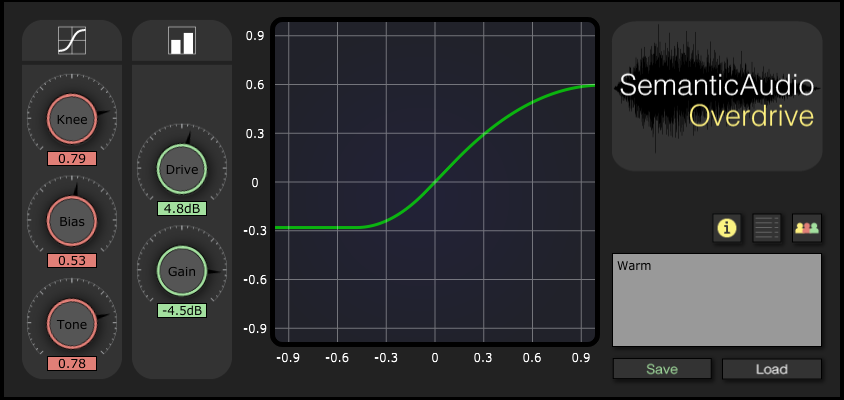
\includegraphics[width=0.8\textwidth]{chapter5/Images/SAFEDistortion.png}
				\caption{The Interface for the SAFE Distortion Plug-In}
				\label{fig:SAFE-Distortion}
			\end{figure}

			The LibXtract library \citep{bullock2007libxtract} is used in the analysis of the audio. Every
			scalar feature available within LibXtract is calculated along with the MFCCs and Bark Band
			Coefficients. In total five seconds of audio is analysed in frames of 4096 samples each.

			\note{Why 4096 samples? The real reason is because LibXtract works better that way. Will that cut
			the mustard?}

			One disadvantage in using plug-ins is that they cannot gather information about the rest of the
			processing chain they may be a part of. The timbral transformation the user is describing my be the
			result of several effects working together. This can be mitigated somewhat by asking users to
			describe only the effect the plug-in in question is providing.

			The SAFE plug-ins also suffer from the same issues other distributed tests do. The researcher
			forfeits control over the listening environment in order to gather results from a much larger sample
			of people. In fact the they provide even lest control that methodologies like that used in the
			Social EQ project \citep{cartwright2013socialeq} in that the choice of audio samples being used is
			decided by the test subject. 
